\section{Side-Channel Attack}
\label{sec:side}

Let us assume gray-box attack context. In practice, there are several means of information leakage, for instance power consumption \cite{kocher1999differential}, electro-magnetic radiation \cite{agrawal2002side,gandolfi2001electromagnetic,quisquater2001electromagnetic}, timing \cite{kocher1996timing}, or even acoustic \cite{asonov2004keyboard} and optical \cite{kuhn2002optical,loughry2002information} emissions may carry some information related to ciphering algorithm's intermediate results or execution. The goal of SCA will be to exploit these information leaks and infer some secrets.

SCA makes use of statistical methods, in cryptography context pioneered by Kocher \cite{kocher1996timing} back in 1996. His paper was originally concentrating on public key cryptography but the idea can be ported to symmetric cryptography as well.

Since then there have been developed several techniques including Simple Power/EM Analysis (SPA/SEMA), Differential Power/EM Analysis (DPA/DEMA), High-Order DPA/DEMA, Correlation Power Analysis (CPA), Inferential Power Analysis (IPA), partitioning attacks, collision attacks, hidden Markov model etc. See \cite[Chapters~13-14]{koc2008cryptographic} for reference.

The success of SCA is based on the following assumptions:
\begin{enumerate}
	\item the cipher is insecure once certain execution-related information leaks (e.g.\ intermediate results or runtime),
	\item the attacker can control, knows or just can predict certain amount of plaintext inputs, and
	\item the attacker has the ability to gain some information related to execution of the cipher.
\end{enumerate}
Let us present this idea on a concrete attack.


% ==============================================================================
% ===   C P A   A T T A C K                                                  ===
% ==============================================================================

\subsection{Correlation Power Analysis Attack}

In this section we describe CPA attack (an advanced form of DPA attack) mounted on an unprotected AES implementation where the attacker can measure power consumption, referred to as {\em power trace}; see Figure \ref{fig:powertrace} for an example power trace. First we show which AES intermediate result leads to immediate key recovery, then we describe how the attacker can utilize information related to this intermediate result hidden in power traces to recover the key. See Algorithm \ref{alg:aes} in Section \ref{sec:aes} for AES construction.

\begin{figure}[h]
\begin{center}
	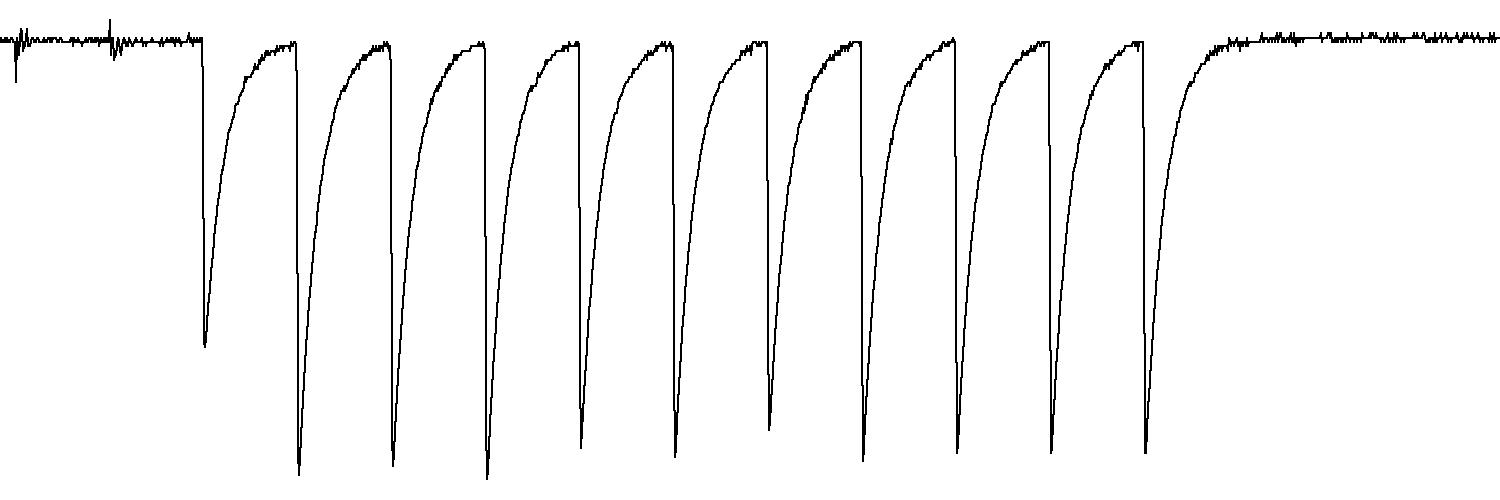
\includegraphics[width=0.9\textwidth]{./figures/power_trace/power_trace.png}
	\caption{SAKURA-G running AES, note its $10$ rounds. Data taken from \cite{exampletraces}.}
	\label{fig:powertrace}
\end{center}
\end{figure}

\subsubsection{Vulnerable Intermediate Result}
	
	In AES (Algorithm \ref{alg:aes}), the very first plaintext-dependent operation is $\AddRoundKey$ on Line \ref{line:addrk} which XORs current state with the first block of expanded key. Here the state is equal to input plaintext, see Line \ref{line:stateplain}, and the first block of expanded key is equal to the original AES key, see Note \ref{note:expkey}. $\AddRoundKey$ is then usually composed with $\SubBytes$ (the following step), hence yielding
	\begin{equation}
		b = \SubBytes(k\xor m) \label{eq:byprod}
	\end{equation}
	as the first intermediate result where $k$ stands for the AES key and $m$ for the plaintext. $b$ is then used in the following AES step which is $\ShiftRows$, usually composed with $\MixColumns$.
		
	Once we knew $b$ and respective $m$ from single AES encryption, it would be easy to directly compute the key as $k = S^{-1}(b)\xor m$.

\subsubsection{Utilizing Power Traces}
	
	But in this attack scenario we do not observe intermediate results $b$ directly, we only have power traces. Now let us describe a reasonable model how certain portion of information about $b$'s leaks into the power trace and how we can exploit it.
	
	Before entering next stages, the intermediate result $b$ is temporarily stored. It is handled byte-wise, hence its byte-wise Hamming weights (i.e.\ numbers of ones in binary representation, further denoted by $HW$) are reflected into the power trace\footnote{Here we assume so called {\em Hamming Weight Leakage Model}.}. It means that for each byte of $b$ denoted by $b_i$ there is a position in the power trace which reflects $HW(b_i)$.
	
	Let us suppose that we have a plenty of such traces which are properly aligned i.e.\ a position in the traces corresponds with a fixed position in the AES implementation. Therefore, for each byte of $b$'s, there is a position in the traces where the power values are correlated with Hamming weights of respective bytes of respective $b$'s.
	
	Since we do not know actual $b$'s, we will assume that the correlation of true values of $b$'s is the highest among others and among all positions in the traces. Note that $b_i = S(k_i\xor m_i)$ i.e.\ $b$'s only depend on respective known plaintexts $m$ and the key $k$ which is constant, therefore we will loop through key guesses and search for globally maximal correlation. And more importantly, note that we can guess the key byte-wise!
	
	\begin{note}
	\label{note:brutevssca}
		In CPA we loop through $256$ key guesses for each of $16$ bytes i.e.\ overall $256\cdot 16 = 2^{12} = 4096$ possibilities, compare with $256^{16} = 2^{128} = \ldots$ possibilities of a brute force attack.
	\end{note}
	
	The attack will perform as follows: given a byte index $i=\atob{0}{15}$, we find the maximal correlation\footnote{We can use an empirical meter as well since correlation is quite expensive and we only need the result, no matter how we reach it.} (among all keyguesses $k_i$ of $i$-th byte of the key and all positions in the traces) of $HW\bigl(S(k_i\xor m_i)\bigr)$ with respective power values. $k_i$ reaching the maximum is then our top candidate. This idea is summarized in the following algorithm.
	
	\begin{alg}
	\label{alg:cpa}
	Given power traces and respective plaintexts, recover the AES key.
		\begin{algorithmic}[1]
			\Function{CPA\_Attack}{$Traces[N][T],PTs[N]$}
				\For{$i = 0 \to 15$}
					\State $max \gets 0$
					\For{$KGuess = \texttt{00} \to \texttt{ff}$}
						\State $tmpmax \gets \max\limits_{t\in T} \Corr\limits_{n\in N}\Bigl(Traces[n][t], HW\bigl(S(KGuess\xor PTs[n][i])\bigr)\Bigr)$
							\label{line:corr}
						\If{$tmpmax > max$}
							\State $max \gets tmpmax$
							\State $BestKey[i] \gets KGuess$
						\EndIf
					\EndFor
				\EndFor
				\State\Return $BestKey$
			\EndFunction
		\end{algorithmic}
	\end{alg}
	
	\begin{remark}
	\label{rem:attacklookup}
		We obviously do not compute SBox and Hamming weight at each step, but rather use a single precomputed table of the composition of $HW\circ S$. Clearly, this table has $256$ entries.
	\end{remark}
	
	\begin{note}
	\label{note:fulllist}
		It is useful to modify the previous algorithm to output the whole list of key candidates together with their maximal correlation values for each key byte i.e.\ the result of Line \ref{line:corr}, not only $BestKey$.
		
		This is because if $BestKey$ is not equal to the true key, we still have a good chance to recover the key: since the true key is likely to have rather high correlation, we loop through key candidates according to their correlation values, higher first.
		
		Note that we can verify correctness of our key guess simply by checking whether the resulting ciphertext equals to the ciphertext we expect.
	\end{note}
	
	\begin{note}
	\label{note:leakpos}
		It might be also helpful to output positions of maximal correlation for each candidate. This information might be valuable for any further analysis purposes.
	\end{note}
	
	There are several solutions implementing CPA including an open-source ChipWhisperer\texttrademark\ Project \cite{chipwhisperer} which is a toolkit providing a complete toolchain from trace acquisition to key extraction. We derived this algorithm from the documentation of ChipWhisperer\texttrademark.


% ==============================================================================
% ===   B I T - W I S E   D P A                                              ===
% ==============================================================================

\subsection{Bit-Wise Differential Power Analysis Attack}

Let us continue with another attack on an unprotected AES implementation. For now, let us suppose a more powerful attacker who can probe individual wires of a vulnerable bus and measure its voltage. Let us further suppose that transfers of intermediate result $b = \SubBytes(k\xor m)$ are transferred over this bus.

Therefore such attacker is not limited to observing values related to Hamming weight of $b$ but she can rather measure values related to individual bits of $b$! The advantage of such attacker is that there suffice much less measurements to successfuly recover the key.

\subsubsection{Attack}
	
	In this attack, we proceed similarly as in the previous one i.e.\ we loop through key guesses for each key byte and compute the respective intermediate results $b_i$, see Algirothm \ref{alg:cpa}. But instead of applying Hamming weight and computing correlation, we perform this attack for each bit individually.
	
	Let say we are interested in $j$-th bit of $i$-th byte. Based on actual key guess $k_i$, we compute $j$-th bit of $b_i = S(k_i\xor m_i)$ for each trace/plaintext pair and partition the traces based on this bit into two sets, let us denote them $S_0$ and $S_1$.
	
	\begin{note}
	\label{note:concattraces}
		Typically we have several traces for a single plaintext and we do not know which of them contains which bit. Actually this does not matter, we can serialize them into a single trace and do not care anymore.
	\end{note}
	
	If the key guess is correct, then there is a position in the traces so that the values are low in traces in $S_0$ and high in traces in $S_1$. We will find this position as the spot of the highest difference of mean values. If the key guess is not correct, there should be no substantial peak in difference of means. Hence the true key should maximize the trace-maximal difference of means among other key guesses. An algorithm implementing this attack follows.
	
	\begin{alg}
	\label{alg:bitwisedpa}
	Given voltage traces and respective plaintexts, recover the AES key.
		\begin{algorithmic}[1]
			\Function{Bitwise\_DPA\_Attack}{$Traces[N][T],PTs[N]$}
				\For{$i = 0 \to 15$}
					\State $max \gets 0$
					\For{$KGuess = \texttt{00} \to \texttt{ff}$}
						\For{$j = 0 \to 7$}\label{line:tbcycle}
							\State $S_0 \gets \Bigl\{ Traces[n] \Bigm| S\bigl(KGuess\xor PTs[n][i]\bigr)[j] = 0 \Bigr\}$ \label{line:s0}
							\State $S_1 \gets \Bigl\{ Traces[n] \Bigm| S\bigl(KGuess\xor PTs[n][i]\bigr)[j] = 1 \Bigr\}$ \label{line:s1}
							\State $tmpmax \gets \max\limits_{t\in T} \Bigl| \Mean\limits_{Trace\in S_1}\bigl(Trace[t]\bigr) - \Mean\limits_{Trace\in S_0}\bigl(Trace[t]\bigr) \Bigr|$
								\label{line:diffmean}
							\If{$tmpmax > max$}
								\State $max \gets tmpmax$
								\State $BestKey[i] \gets KGuess$
							\EndIf
						\EndFor
					\EndFor
				\EndFor
				\State\Return $BestKey$
			\EndFunction
		\end{algorithmic}
	\end{alg}
	
	\begin{note}
	\label{note:eightlists}
		We can modify this algorithm in a manner similar to Note \ref{note:fulllist} and \ref{note:leakpos} to output the full record of maximal differences of means (instead of correlations previously, here it is the result of Line \ref{line:diffmean}) and their positions in traces. Note that in this case we get $8$ separate lists for each $j$, see Line \ref{line:tbcycle} in the previous algorithm. Here $j$ is referred to as {\em target bit}. We can also unravel which target bit leaks the most which might be useful for further analysis purposes.
	\end{note}
	
	%!% prověřit
	To the best of our knowledge, there is no open-source project implementing this attack. This method has been taken from \cite{teuwen2015movfuscator}.

% tabulku korelací na základě hamming weight?
